%%%%%%%%%%%%%%%%%%%%%%%%%%%%%%%%%%%%%%%%%
% Friggeri Resume/CV
% XeLaTeX Template
% Version 1.1 (9/2/15)
%
% This template has been downloaded from:
% http://www.LaTeXTemplates.com
%
% Original author:
% Adrien Friggeri (adrien@friggeri.net)
% https://github.com/afriggeri/CV
%
% License:
% CC BY-NC-SA 3.0 (http://creativecommons.org/licenses/by-nc-sa/3.0/)
%
% Important notes:
% This template needs to be compiled with XeLaTeX and the bibliography, if used,
% needs to be compiled with biber rather than bibtex.
%
%%%%%%%%%%%%%%%%%%%%%%%%%%%%%%%%%%%%%%%%%

\documentclass[]{friggeri-cv} % Add 'print' as an option into the square bracket to remove colors from this template for printing
\addbibresource{bibliography.bib} % Specify the bibliography file to include publications
% !BIB TS-program = biber
%%%%%%%%%%%%%% copied form line 163 in friggeri-cv
% Side block %
%%%%%%%%%%%%%%»
\RequirePackage[absolute,overlay]{textpos}

\renewenvironment{aside}{%
  \let\oldsection\section
  \renewcommand{\section}[1]{
    \par\vspace{\baselineskip}{\Large\headingfont\color{headercolor} ##1}
  }
  \begin{textblock}{4.6}(0.5, 4.33)
  \textblockcolour{white}    % this line is here to help you and then should be removed
  \begin{flushright}
  \obeycr
}{%
  \restorecr
  \end{flushright}
  \end{textblock}
  \let\section\oldsection
}

\geometry{right=0.8cm}

\begin{document}

\header{Dr. Avit K. }{Bhowmik}{Environmental Scientist | Climate Solutionist} % Your name and current job title/field
\smash{\raisebox{-0.41\height\hspace{-180pt}}{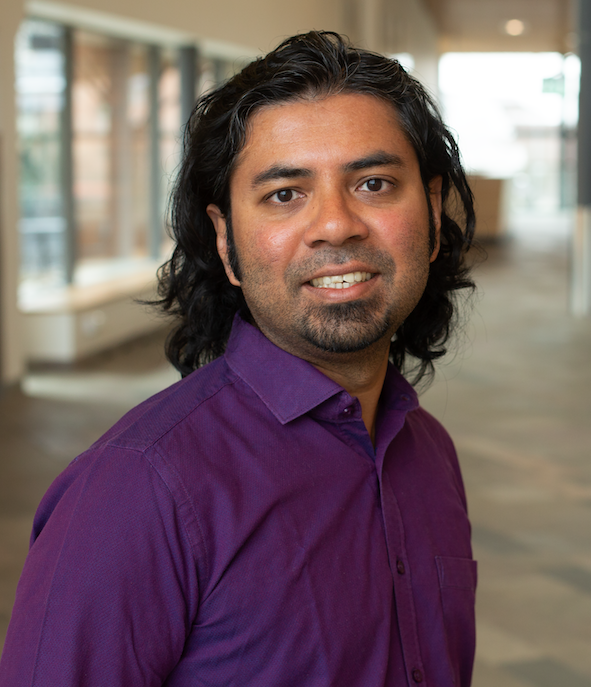
\includegraphics[scale=0.67, bottom]{photo.png}}}


%----------------------------------------------------------------------------------------
%	SIDEBAR SECTION
%----------------------------------------------------------------------------------------

\begin{aside} % In the aside, each new line forces a line break
~
Born on 27 September, 1986
~
\section{contact}
\vspace{5pt}\small{
Risk and Environmental Studies
Karlstad University
Universitetsgatan 2
SE 651 88 Karlstad, Sweden
~
Tel: +46 (0)54 700 10 44
Fax: +46 (0)54 700 10 44
~
E-mail: \href{mailto:avit.bhowmik@kau.se}{avit.bhowmik@kau.se}
Web: \href{http://avitbhowmik.com/}{\small{http://avitbhowmik.com/}
Publications: \href{https://scholar.google.com/citations?hl=en&user=laRo5pgAAAAJ}{\small{Google Scholar}}}
~
\section{research areas}
\vspace{5pt}Sustainability transformation
Climate action
Social tipping points
Agency and Scale of Action
Geostatistics
~
\section{technical skills}
\vspace{5pt} \textbf{Programing \& Modelling}
R, C++, Python, Netlogo and Unix Shell'
%------------------------------------------------
\vspace{5pt}\textbf{Databases}
SQL and PostgreSQL
%------------------------------------------------
\vspace{5pt}\textbf{Geoinformatics}
GRASS GIS, Quantum GIS, ArcGIS, GeoMS, and ERDAS IMAGINE
%------------------------------------------------
\vspace{5pt}\textbf{Communication and Presentation}
HTML, CSS, MarkDown and \LaTeX
%------------------------------------------------
~
\section{languages}
\vspace{5pt}Bangla: mother tongue
English: level C2
Swedish: level B1
German: level C1
Portuguese: level A1

\vspace{10pt} \tiny{(Levels: A1/2: Basic user - B1/2: Independent user - C1/2: Proficient user, according to Common European Framework of Reference for Languages)}}

\end{aside}

%----------------------------------------------------------------------------------------
% KEY ACHIEVEMENTS SECTION
%----------------------------------------------------------------------------------------
\section{key achievements}

\begin{entrylist}
%------------------------------------------------
\entry
{\small{2024 - present}}
{Successful research grant from Vinnova (Swedish Innovation Agency)}
{}
{Main applicant (PI) of the project ``Development of sustainability Indicators to drive innovation for Energy Transition (DIET) in Värmland''(200 000 euro).}
%------------------------------------------------
\entry
{\small{2024 - present}}
{Successful research grant from Swedish Energy Agency and Viable Cities}
{}
{Co-applicant with Arvika Municipality, Sweden, of the project ``Climate Neutral Arvika 2030''(500 000 euro).}
%------------------------------------------------
\entry
{\small{2024 - present}}
{Successful grant by the Swedish Agency for Economic and Regional Growth (co-financed by European Union)}
{}
{Co-applicant and major contributor to the work-packages on ``Energy Communities'' and ``Local Energy Leadership'' of the project ``Local Energy Leadership in Värmland (LOKEN)''(2 M euro).}
%------------------------------------------------
\entry
{\small{2022 - present}}
{Advisor to \href{https://acba.africa}{``African Circular Business Alliance''}}
{}
{Advising and assisting African Circular Business Alliance in developing sustainable and circular business models for rapidly reducing greenhouse gas emissions}
%------------------------------------------------
\entry
{\small{2022 - present}}
{Successful European Commission Erasmus+ grant}
{}
{Co-applicant and co-leader of the work-package establishing cooperation between government and academia to develop tools and guides for strengthening policies, of the project grant ``Alliance of regional innovation ecosystems based on smart sustainable specialization strategies (ARIES4)'' (1.38 M euro).}
%------------------------------------------------
\entry
{\small{2020 - present}}
{Advisor to \href{https://www.forshaga.se/jobbochforetagande/startaochdrivaforetag/natverkochsamarbeten/natverkethallbaragenda.4.491d250d1775b5bab0279483.html}{``Sustainability Agenda''} of Forshaga and Munkfors municipalities}
{}
{Advising and assisting Forshaga and Munkfors municipalities in developing disrupting emissions reduction strategies for business and industries to achieve climate neutrality by 2040}
%------------------------------------------------
\entry
{\small{2020}}
{PNAS article: Social tipping dynamics for stabilizing Earth’s climate by 2050}
{}
{Co-led the development of the concept ``Social Tipping Points'' and outlined six key interventions that can contagiously and rapidly transform global societies for climate action. See \href{http://www.pnas.org/content/early/2020/01/14/1900577117.abstract}{here} for details.}
%------------------------------------------------
\entry
{\small{2018 - 2019}}
{\href{https://exponentialroadmap.org}{Exponential Climate Action Roadmap}} 
{}
{Led the research and modelling exercises to lay out the first exponential pathways for climate action to halve greenhouse gas emission every decade from 2020 through 2050. The first output report was highlighted in \href{https://www.globalclimateactionsummit.org}{Global Climate Action Summit}, held in San Francisco, September 2018, and an update was released during the \href{https://www.un.org/en/climatechange/un-climate-summit-2019.shtml}{UN Climate Action Summit 2019}.}
%------------------------------------------------
\entry
{\small{2018}}
{\href{http://www.iiasa.ac.at/web/home/research/twi/TWI2050.html}{The World in 2050}} 
{}
{Contributed to shape the narrative and pathways for achieving the Sustainable Development Goals of the ``Agenda 2030'', led by United Nations Sustainable Development Solutions Network (SDSN), the output reports of which have been regularly presented in \href{https://sustainabledevelopment.un.org/hlpf/2018}{United Nations High Level Political Forums}.}
%------------------------------------------------
\end{entrylist}
\section{}
\begin{entrylist}
\entry
{\small{2017}}
{European Research Council (ERC) Advanced Grant} 
{}
{Co-applicant and contributed with drafting, reviewing and transformation, social tipping points and geospatial research expertise to a successful ERC Advanced grant proposal, i.e. ``Earth Resilience in the Anthropocene (ERA)'' (2,500,000 euro), Principal Investigator: Prof. Dr. Johan Rockström.}
%------------------------------------------------
\entry
{\small{2016}}
{Arctic Science Ministerial Report} 
{}
{Provided expert opinion for spatiotemporal variability modelling of climate and resilience in the Arctic, which shaped the policy framework of the ``U.S.-Canada Joint Statement on Climate, Energy, and Arctic Leadership'' in the first White House Arctic Science Ministerial Meeting on September 28, 2016.}
%------------------------------------------------
\end{entrylist}

%----------------------------------------------------------------------------------------
% EDUCATION SECTION
%----------------------------------------------------------------------------------------
\section{education}

\begin{entrylist}
%------------------------------------------------
\entry
{\small{06/2026 (exp.)}}
{Docent (Appointment as a University Reader)}
{Karlstad University, Sweden}
{Risk and Environmental Studies, Faculty of Arts and Social Sciences}
%------------------------------------------------
\entry
{\small{09/2012--12/2015}}
{Doctor of Natural Sciences}
{University of Koblenz-Landau, Germany}
{Quantitative Landscape Ecology, Institute for Environmental Sciences\\
Dissertation: {\emph{Human and Ecological Impacts of Freshwater Degradation on Large Scales. Development and Integration of Spatial Models with Ecological Models for Spatial-ecological Analyses} (supervisor: Prof. Dr. Ralf B. Sch\"afer)} \\
Specialization: Spatial Statistics, Freshwater Eco(toxico)logy, Climate\\
Grade: 1.0 (top ranked) on a scale of 1.0 - 3.0 (1.0 best and 3.0 sufficient)}
%------------------------------------------------
\entry
{\small{09/2010--03/2012}}
{Master of Science {\normalfont{\footnotesize{in Geospatial Technologies}}}}
{Erasmus Mundus, European Commission}
{Partners: 1. School of Statistics and Information Management, New University of Lisbon, Portugal, 2. Institute for Geoinformatics (ifgi), University of M\"unster, Germany and 3. Department of Computer Languages and Systems, University of Jaume I, Spain\\
Dissertation: {\emph{Evaluation of Spatial Interpolation Techniques for Mapping Climate Variables with low sample density. A case study using a new gridded dataset of Bangladesh} (supervisor: Prof. Dr. Ana Cristina Costa)} \\
Major: Geostatistics, Geographic Information Science (GIS), Climate \\
Grade: 18 (top ranked) on a scale of 1 - 20 (20 best and 1 worst)}
%------------------------------------------------
\entry
{\small{12/2004--10/2009}}
{Bachelor of Science {\normalfont{\scriptsize{in Urban \& Regional Planning}}}}
{\scriptsize{Bangladesh University of Engineering \& Technology}}
{Department of Urban \& Regional Planning\\
Dissertation: {\emph{Relocation of the Hazaribagh Tannery: Myth or Reality?} (supervisor: Prof. Dr. Md. Shakil Akther)}\\
Major: GIS, Environmental and Ecological Planning \\
Grade: 3.79 on a scale of 0-4.0 (4.0 best and 0 worst)}
%------------------------------------------------
\end{entrylist}

%----------------------------------------------------------------------------------------
%	WORK EXPERIENCE SECTION
%----------------------------------------------------------------------------------------
\section{professional experience}

\begin{entrylist}
%------------------------------------------------
\entry
{\small{03/2019--present}}
{Assistant Professor}
{Karlstad University, Sweden}
{Risk and Environmental Studies\\
15\% teaching and 85\% research\\
Karlstad University Representative: \href{https://www.unsdsn-ne.org/en}{Sustainable Development Solutions Network Northern Europe}}
%------------------------------------------------
\end{entrylist}
\section{}
\begin{entrylist}
\entry
{\small{01/2018--02/2019}}
{Postdoctoral Researcher \& Liaison}
{Royal Swedish Academy of Sciences}
{Future Earth \\
1. \href{https://x-cac.futureearth.org/} {Exponential Climate Action} project: Backcasting modelling of climate action strategies to achieve Paris Agreement following the Carbon Law\\
2. \href{http://www.iiasa.ac.at/web/home/research/twi/TWI2050.html} {The World in 2050} project: Geospatial modelling and spatiotemporal analyses of drivers and processes underlying Sustainable Development Goals\\
3. Secretariat Liaison: Global Research Projects: (i) Analysis, Integration and Modelling of the Earth System (AIMES) and (ii) Integrated History and Future of People On Earth (IHOPE), and Knowledge Action Networks: (i) Decarbonization and (ii) Sustainable Development Goals}
%------------------------------------------------
\entry
{\small{01/2018--02/2019}}
{Guest Researcher}
{Stockholm University, Sweden}
{Stockholm Resilience Centre (Planetary Boundaries)}
%------------------------------------------------
\entry
{\small{01/2016--12/2017}}
{Postdoctoral Researcher}
{Stockholm University, Sweden}
{Stockholm Resilience Centre (Planetary Boundaries) \\
Cross-scale dynamics and spatial resilience patterns in social-ecological domains (led by Prof. Dr. Johan Rockstr\"om)}
%------------------------------------------------
\entry
{\small{01/2016--03/2018}}
{Guest Lecturer}
{University of Koblenz-Landau, Germany}
{Courses: 1. GIS Application, 2. GIS Projects for Advanced, 3. Introduction to open-source software and R for spatial ecotoxicological analyses, and 4. Spatial(-Temporal) Interpolation with R}
%------------------------------------------------
\entry
{\small{11/2015--12/2015}}
{Research Assistant}
{University of Koblenz-Landau, Germany}
{Quantitative Landscape Ecology, Institute for Environmental Sciences\\
Project - AufLand: Understanding effects of land use on the energy transfer across the freshwater-land interface}
%------------------------------------------------
\entry
{\small{04/2012--07/2012}}
{Research Assistant}
{University of M\"unster, Germany}
{Institute for Geoinformatics (ifgi)\\
Development of online demonstrators and web tools for core concepts of spatial information}
%------------------------------------------------
\entry
{\small{03/2008--10/2010}}
{Project Assistant}
{Technical University of Dortmund, Germany}
{{\emph{The Struggle for Urban Livelihoods and the Quest for a Functional City Reconciling Informal and Statutory Planning Institutions in Dhaka, Bangladesh,}} supported by the German Research Foundation (DFG) and conducted by the Department of Urban and Regional Planning, Faculty of Spatial Planning\\
Preparation of Geographic Information Systems (GIS) databases, analyses and processing of empirical data, conduction of empirical field investigation, i.e. key informant interviews, group discussion, household interviews and exercise of Venn-diagrams and observations}
%------------------------------------------------
\end{entrylist}


%----------------------------------------------------------------------------------------
% RESEARCH PORTFOLIO SECTION
%----------------------------------------------------------------------------------------
\section{research activities}

%----------------------------------------------------------------------------------------
% RESEARCH VISITS SECTION
%----------------------------------------------------------------------------------------

\section{research visits}

\begin{entrylist}
%------------------------------------------------
\entry
{\small{03/2018--04/2018}}
{Visiting Scholar}
{International Institute for Applied Systems Analysis (IIASA)}
{Energy Program \\
Regional disparities among the trade-offs and co-benefits in the underlying processes of Sustainable Development Goals}
%------------------------------------------------
\end{entrylist}

%----------------------------------------------------------------------------------------
% GRANT SECTION
%----------------------------------------------------------------------------------------
\newpage
\section{Third Party Projects and Grant Volume}
\textbf{Avit Bhowmik}\\

\begin{entrylist}
%------------------------------------------------
\entry
{\small{2021}}
{Climate Game Changers - Gamification for the empowerment to adapt to climate change}
{PIs: Caroline Bhowmik and Prince D´Costa}
{MIRAI 2024-2026 – Joint seed funding of Japan-Sweden collaborative projects\\
Total grant: 10,000 euro\\
Mentor and co-applicant}
%------------------------------------------------
\entry
{\small{2024}}
{Development of sustainability Indicators to drive innovation for Energy Transition (DIET) in Värmland}
{PI: Avit Bhowmik, Karlstad University}
{Vinnova (Swedish Innovation Agency) Grant: 2024-03767\\
Total grant: 200 000 euro\\
Main applicant (PI) and Project Leader}
%------------------------------------------------
\entry
{\small{2024}}
{Climate Neutral Arvika 2030}
{Co-applicant with Arvika Municipality, Sweden}
{Swedish Energy Agency and Viable Cities Grant:P2024-02116 \\
Total grant: 500 000 euro\\
Principal Scientist of the project}
%------------------------------------------------
\entry
{\small{2024 - present}}
{LOKEN - Local Energy Leadership in Värmland}
{}
{Swedish Agency for Economic and Regional Growth (co-financed by European Union), Grant: 20363786\\
Total grant: 2 M euro\\
Co-applicant and major contributor to the work-packages on ``Energy Communities'' and ``Local Energy Leadership''}
%------------------------------------------------
\entry
{\small{2022}}
{Alliance of regional innovation ecosystems based on smart sustainable specialization strategies (ARIES4)}
{Coordinator: Universidad Pública de Navarra (UPNA)}
{European Commission Erasmus+ Grant: 101056369\\
Total grant: 1.38 M euro\\
Contribution: Work-package establishing cooperation between government and academia to develop tools and guides for strengthening policies}
%------------------------------------------------
\entry
{\small{2021}}
{MIRAI2.0 – Joint seed funding of Japan-Sweden collaborative projects}
{PIs: Avit Bhowmik and Shunsuke Managi}
{Total grant: 13,400 euro\\
Startup grant for the research project ``Marketing technology (MARTECH) for customer behavioral transformation to rapidly reduce food wastes''}
%------------------------------------------------
\entry
{\small{2020}}
{Faculty of Arts and Social Sciences Research Advancement Grant}
{PI: Avit Bhowmik}
{Total grant: 36,000 euro\\
Startup grant for research projects}
%------------------------------------------------
\entry
{\small{2020}}
{Exponential Climate Action Roadmap for cities (ExAct)}
{PI: Dr. Avit K. Bhowmik}
{Faculty of Arts and Social Sciences\\
Total grant: 8,000 euro\\
Startup grant for a research project}
%------------------------------------------------
\entry
{\small{2018}}
{How to develop cross-scale and target seeking transformation scenarios through participatory processes?}
{PI: Avit Bhowmik}
{Bolin Centre for Climate Research\\
Total grant: 9,000 euro\\
Seed grant for pilot research projects on Sustainable Development Goals}
%------------------------------------------------
\entry
{\small{2017}}
{Social-ecological Resilience in the Anthropocene}
{PI: DAvit Bhowmik}
{Department of Biology, Stockholm University\\
Total grant: 4,200 euro\\
Supported and supervised three master's theses projects}
%------------------------------------------------
\end{entrylist}
\section{}
\begin{entrylist}
\entry
{\small{2016}}
{Earth Resilience in the Anthropocene (ERA)}
{Co-applicant, PI: Prof. Dr. Johan Rockström}
{European Research Council (ERC) Advanced Grant\\
Total grant: 2,500,000 euro\\
Contributions: (a) wrote and reviewed the grant proposal, (b) led work packages 2 \& 4, (c) added geospatial research expertise}
%------------------------------------------------
\entry
{\small{2012--2015}}
{Quantitative Landscape Ecology Ph.D. Grant}
{PI: Avit Bhowmik}
{University of Koblenz-Landau, Germany\\
German Research Foundation (DFG) supported project\\
Total grant: 36,000 euro}
%------------------------------------------------
\entry
{\small{2010--2012}}
{Erasmus Mundus Scholarship}
{}
{{\emph{Master of Science in Geospatial Technology}} \\
The Education, Audiovisual and Culture Executive Agency (EACEA), European Commission\\
Total grant: 24,000 euro}
%------------------------------------------------
\end{entrylist}

%----------------------------------------------------------------------------------------
% Algorithm development SECTION
%----------------------------------------------------------------------------------------
\newpage
\section{models \& software development}

\begin{entrylist}
%------------------------------------------------
\entry
{\small{10/2012}}
{ATRIC}
{}
{Automated Accumulation Threshold selection and RIparian Corridor delineation \\
Developed by co-interfacing R and GRASS GIS \\
Development page: \href{https://github.com/AvitBhowmik/ATRIC}{https://github.com/AvitBhowmik/ATRIC}}
%------------------------------------------------
\entry
{\small{08/2011}}
{SSTP}
{}
{Spatially Shifting Temporal Points \\
Developed using the gstat package utilities in R \\
Development page: \href{https://github.com/AvitBhowmik/SSTP}{https://github.com/AvitBhowmik/SSTP}}
%------------------------------------------------
\end{entrylist}

%----------------------------------------------------------------------------------------
% Leadership Skills SECTION
%----------------------------------------------------------------------------------------
\section{administrative positions and duties}

\begin{entrylist}
%------------------------------------------------
\entry
{\small{01/2018--present}}
{Research Director}
{Karlstad University}
{\href{https://www.kau.se/en/crs}{Centre for Sustainable Societal Transformation}}
%------------------------------------------------
\entry
{\small{03/2019 - present}}
{Course Director and Developer}
{Karlstad University}
{CCGA08: Nordic Climate Change Studies\\
CCGA01: Sustainable Development with a focus on Climate Change\\
RHG310: Climate Change Adaptation and Mitigation\\
MVG300: Environment, Risk and Sustainable Development}
%------------------------------------------------
\entry
{\small{01/2018--present}}
{Lead Researcher}
{\href{https://exponentialroadmap.org}{Exponential Roadmap Initiative}}
{Lead partners: IKEA, WWF, Finnish Innovation Fund, Mission 2020}
%------------------------------------------------
\entry
{\small{09/2021}}
{Principal Organizer}
{}
{Book Seminar: Under the Sky We Make. How to be Human in a Warming World\\
by Dr. Kimberly Nicholas from Centre for Sustainability Studies, Lund University\\
Centre for Sustainable Societal Transformation, Karlstad University, Sweden}
%------------------------------------------------
\entry
{\small{04/2018}}
{Principal Organizer}
{}
{Workshop: Exponential Climate Action for Cities, Carbon Law Accelerator project, Future Earth, Stockholm, Sweden}
%------------------------------------------------
\entry
{\small{02/2018}}
{Theme Leader}
{}
{Pathways to new collaborations in climate research at Stockholm University: Perspectives from the Human Science Academic Area and the Bolin Centre for Climate Research}
%------------------------------------------------
\entry
{\small{08/2017}}
{Session Chair}
{}
{Session: Exploring the potential of local innovations and bottom-up change, Social-ecological transformations for sustainability, Resilience 2017 - Resilience Frontiers for Global Sustainability}
%------------------------------------------------
\end{entrylist}
\section{}
\begin{entrylist}
\entry
{\small{06/2017}}
{Principal Organizer}
{}
{Workshop: Progress in computational macroecology, The 17th International Conference on Computational Science and Its Applications (ICCSA 2017), Trieste, Italy}
%------------------------------------------------
\entry
{\small{12/2016}}
{Principal Organizer}
{}
{Social Tipping Elements Instrumental for Decarbonization by 2050: an Expert Workshop, The Earth League, Stockholm Resilience Centre, Sweden}
%------------------------------------------------
\entry
{\small{09/2016}}
{Co-organizer}
{}
{Climate Tipping Points and Safe Pathways to Sustainable Development: an expert review workshop, Stockholm Resilience Centre, Stockholm, Sweden\\
Analysis, Integration and Modelling of the Earth System (AIMES)}
%------------------------------------------------
\entry
{\small{05/2016}}
{Principal Organizer}
{}
{3rd Earth-Doc Meeting, Stockholm Resilience Centre, Sweden\\
(a) Preparation of a strategy document outlining Earth-Doc research, and (b) Advancing on the on-going Earth-League research proposal and perspective paper}
%------------------------------------------------
\entry
{\small{07/2015}}
{Principal Organizer}
{}
{Workshop 1: Data analysis in freshwater ecology using R, 9th Symposium for European Freshwater Sciences (SEFS), Geneva, Switzerland}
%------------------------------------------------
\entry
{\small{09/2012--12/2015}}
{Developer and Maintainer}
{}
{Geodata Server \\ 
Institute for Environmental Sciences, University of Koblenz-Landau, Germany}
%------------------------------------------------
\entry
{\small{11/2010--02/2011}}
{Group Leader}
{}
{Spatial statistics group \\ 
Group project seminar on Identifying optimal location for disaster evacuation centres in Lisbon, New University of Lisbon, Portugal}
%------------------------------------------------
\entry
{\small{07/2007--present}}
{U.S. Department of State Alumni}
{}
{Study of the United States Institute for Student Leaders 2007, organized by the United States Department of State in Washington and Green River Community College, Seattle, USA\\
Community services}
%------------------------------------------------
\end{entrylist}


%----------------------------------------------------------------------------------------
% EDITORIAL SECTION
%----------------------------------------------------------------------------------------
\section{editorial activities}

\begin{entrylist}
%------------------------------------------------
\entry
{\small{2018--2019}}
{Guest Editor}
{}
{Sustainability Science}
%------------------------------------------------
\entry
{\small{2016--2019}}
{Reviewer for research project grants}
{}
{Future Earth Sustainable Development Goals Labs\\
Chilean National Science and Technology Commission}
%------------------------------------------------
\entry
{\small{2016--present}}
{Editorial board member}
{}
{Water Science and Technology: Water Supply}
%------------------------------------------------
\entry
{\small{2014--present}}
{Ad-hoc reviewer}
{}
{Nature: Communications Earth \& Environment\\
Nature: npj Urban Sustainability\\
Global Ecology and Biogeography\\
Ecography\\
International Journal of Climatology\\
Sustainability}
\end{entrylist}
\section{}
\begin{entrylist}
\entry
{}
{}
{}
{PLOS ONE\\
Earth Science Informatics\\
Geomatics, Natural Hazards and Risk\\
Journal of Environmental Informatics\\
Applied Ecology and Environmental Research\\
Journal of Health and Pollution\\
Natural Hazards\\
Geosciences\\
Geoscience Data Journal\\
Environmental Monitoring and Assessment\\
International Journal of Environmental Research and Public Health\\
Agronomy\\
Geomorphology}

\end{entrylist}

%\newpage

%----------------------------------------------------------------------------------------
% NETWORKS
%----------------------------------------------------------------------------------------
\section{science-policy-industry networks}

\begin{entrylist}
%------------------------------------------------
\entry
{\small{2022--present}}
{Analysis, Integration and Modelling of the Earth System (AIMES)}
{}
{Scientific Steering Committee Member}
%----------------------------------------------------------------------------------------
\entry
{\small{2020--present}}
{Forshaga and Munkfors municipalities, Sweden}
{}
{Project: \href{https://www.forshaga.se/jobbochforetagande/startaochdrivaforetag/natverkochsamarbeten/natverkethallbaragenda.4.491d250d1775b5bab0279483.html}{Sustainability Agenda}. Development of a Climate Action Framework to achieve carbon neutrality by 2045}
%------------------------------------------------
\entry
{\small{2016--2019}}
{Earth-Doc, \href{http://www.the-earth-league.org/earth-doc-bios.html}{The Earth League}}
{}
{Project: Earth Lander - Social tipping elements instrumental for decarbonization by 2050}
%------------------------------------------------
\entry
{\small{2016--2018}}
{European Space Agency}
{}
{Project: \href{http://earthsystemdatacube.net/}{Earth System Data Cube}, partners: Brockmann Consultant Gmbh, Max Planck Institute for Biogeochemistry and Stockholm Resilience Centre}
%------------------------------------------------
\entry
{\small{2016--present}}
{Sustainable Development Solutions Network (SDSN)}
{}
{Project: The World in 2050 (TWI 2050)}
%----------------------------------------------------------------------------------------
\entry
{\small{2015--2020}}
{European Geosciences Union (EGU)}
{}
{Member}
%----------------------------------------------------------------------------------------
\entry
{\small{2013--2016}}
{Society of Ecotoxicology and Chemistry (SETAC)}
{}
{Member}
%----------------------------------------------------------------------------------------
\end{entrylist}

%----------------------------------------------------------------------------------------
% Jury SECTION
%----------------------------------------------------------------------------------------

\section{jury and examination}

\begin{entrylist}
%------------------------------------------------
\entry
{\small{10/2021}}
{Licentiate Defence Opponent}
{}
{Risk and resilience: An integrated approach for navigating a complex world\\
Emmy Wassénius, Doctoral dissertation \\
Stockholm Resilience Centre, Stockholm University, Sweden and \\
Global Economic Dynamics and the Biosphere, Royal Swedish Academy of Science, Sweden}
%------------------------------------------------
\entry
{\small{07/2021}}
{Ph.D. Defence Jury}
{}
{GIS Applications on the Essential Public Services in Mozambique\\
António Dos Anjos Luis, Doctoral dissertation \\
Nova Information Management School, New University of Lisbon, Portugal}
%------------------------------------------------
\end{entrylist}

%----------------------------------------------------------------------------------------
% PUBLICATIONS SECTION
%--------------------------------------------------------------------------------
\newpage
\section{publications, presentations, outreach}
\section{bibliographic metrics}

\begin{entrylist}
%------------------------------------------------
\entry
{\textbf{h-index: 24}}
{\hspace{10pt}i10-index: 30\hspace{35pt} 3111 citations since 2012}
{source: {\href{https://scholar.google.de/citations?user=laRo5pgAAAAJ&hl=en}{google scholar}}}

\end{entrylist}

\begin{refsection}
\nocite{*}
\printbibliography[type={article}, keyword={workpaper}, title={working papers}, heading=subbibliography]
\end{refsection}

\begin{refsection}
\nocite{*}
\printbibliography[type={article}, notkeyword={workpaper}, title={peer reviewed journal articles}, heading=subbibliography]
\end{refsection}
%\printbibsection{article}{peer reviewed journal articles} % Print all articles from the bibliography
\begin{refsection}
\nocite{*}
\printbibliography[type={incollection}, title={books and book chapters}, heading=subbibliography]
\end{refsection}
%\printbibsection{incollection}{books and book chapters} % Print all books from the bibliography
%\newpage
\printbibsection{report}{reports \& policy papers} % Print all reports from the bibliography
\begin{refsection}
\nocite{*}
\printbibliography[type={inproceedings}, keyword={confpaper}, title={conference papers}, heading=subbibliography]
\end{refsection}
%----------------------------------------------------------------------------------------
%----------------------------------------------------------------------------------------
% Presentation SECTION
%----------------------------------------------------------------------------------------

\section{presentations}
\begin{refsection}
\nocite{*}
\printbibliography[type={inproceedings}, keyword=invpres, title={invited presentations}, heading=subbibliography]
\end{refsection}

\begin{refsection}
\nocite{*}
\printbibliography[type={inproceedings}, keyword=presconf, title={conference presentations \& abstracts}, heading=subbibliography]
\end{refsection}

%------------------------------------------------

%----------------------------------------------------------------------------------------
% Popular science SECTION
%----------------------------------------------------------------------------------------
%\vspace{16pt}
%\section{communication \& outreach}
%\vspace{-16pt}
\begin{refsection}
\nocite{*}
\printbibliography[type={inproceedings}, keyword=communication, title={communication \& outreach}, heading=subbibliography]
\end{refsection}

%------------------------------------------------

\newline
\vspace{1cm}
\normalfont{Karlstad, \today}}
\newline

\includegraphics[width=0.18\linewidth]{signature.png}\\
\textbf{Avit K. Bhowmik}

\end{document}